\documentclass[aps,twocolumn,secnumarabic,nobalancelastpage,amsmath,amssymb,
nofootinbib,superscriptaddress]{revtex4-1}


\usepackage{graphics}       % standard graphics specifications
\usepackage{graphicx}       % alternative graphics specifications
\usepackage{longtable}      % helps with long table options
\usepackage{url}            % for on-line citations
\usepackage{bm}             % special 'bold-math' package
\usepackage[ngerman]{babel} % deutsche Siblentrennung
\usepackage[utf8]{inputenc} % Umlaute

\def\andname{\hspace*{-0.5em},} % definiert die Trennung zwischen 2 Autoren neu
\setlength\parindent{0pt} % kein indent

% Titelseite
\begin{document}
\title{Quantisierter Leitwert von Punktkontakten}
\author         {Ch. Egerland}
\email[Email: ]{egerlanc@physik.hu-berlin.de}
\author         {M. Pfeifer}
\email[Email: ]{max.pfeifer@physik.hu-berlin.de}
\affiliation    {Humboldt-Universität zu Berlin, Institut für Physik}
\date[Versuchsdatum: ]{22.06.2017}

%%%%%%%%%%%%%%%%%%%%%%%%%%%%%%%%%%%%%%%%%%%%%%%%%%%%%%%%%%%%%%%%%%%%%%%%%%%%%%%%
\begin{abstract}
Der ballistische Transport von Elektronen eines zweidimensionalen Fermigases in einem
GaAs-AlGaAs Punktkontakt wurde bereits 1987 von Wees et. al  \cite{wees88} untersucht.
Es wird versucht die Ergebnisse dieses Experimentes zu reproduzieren. Hierbei wird
zunächst eine verkürzte Herleitung des Phänomens beschrieben, über die Aufnahme
der Daten und deren Analyse berichtet und danach über die Unsicherheiten des Experimentes
diskutiert.
\end{abstract}


\maketitle



%%%%%%%%%%%%%%%%%%%%%%%%%%%%%%%%%%%%%%%%%%%%%%%%%%%%%%%%%%%%%%%%%%%%%%%%%%%%%%%%

\section{Theorie}

Der Leitwert ist das Inverse des Widerstandes und ist ein Maß dafür, wie gut ein
Material Strom leitet. Die Quantisierung des Leitwertes kann wie folgt erklärt
werden: Wir modellieren den Quantenpunktkontakt als ein effektives Kastenpotential
mit Breite $d_x$ und Dicke $d_y$. Es bilden sich senkrecht zur Bewegungsrichtung
stehende Elektronenwellen mit der folgenden Energie aus:

  \begin{equation}
    E_{lm} = \frac{\pi^2 \hbar^2}{2 m_e} \left(\frac{l^2}{d_x^2}+\frac{m^2}{d_y^2} \right)
  \end{equation}

In Bewegungsrichtung haben wir unter den Voraussetzungen ein kontinuierliches
Energiespektrum mit $E_z = \hbar^2 k_z^2 / 2m_e$. Die Gesamtenergie der elektronischen
Zustände ist dann: $E_{ges} = E_{lm} + E_z$.
Die Zustandsdichte in einem eindimensionalen System ist gegeben durch:

  \begin{equation}
    D(E) \mathrm{d}E = \frac{1}{\pi \hbar} \sqrt{\frac{m}{2 E}}\mathrm{d}E
  \end{equation}

Bei Anlegen einer kleinen Spannung $\mathrm{d}V$ folgt ein kleiner Strom $\mathrm{d}I = e v \mathrm{d}n$,
wobei $\mathrm{d}n = D(E)\mathrm{d}E$. Somit ist (mit $v = \sqrt{2E/m}$):

  \begin{equation}
    G = \frac{\mathrm{d}I}{\mathrm{d}V} = \frac{evD(E)\mathrm{d}E}{\mathrm{d}V} = \frac{e^2vD(E)\mathrm{d}V}{\mathrm{d}V} = \frac{2e^2}{h}
  \end{equation}






%%%%%%%%%%%%%%%%%%%%%%%%%%%%%%%%%%%%%%%%%%%%%%%%%%%%%%%%%%%%%%%%%%%%%%%%%%%%%%%%
\section{Experiment}

Das Experiment ist bebildert in \cite{skript11} erklärt und besteht im Wesentlichen
aus einem Lock-In-Verstärker an den zunächste zwei Transformatoren sowie die
Widerstandsbox angeschlossen sind. Nun wird überprüft, ob der gemessene Widerstand
dem angeschlossenen Widerstand entspricht. Die Abweichung vom Idealfall dient uns
dann als systematischer bzw. zufälliger Fehler (weiteres hierzu in Abschnitt III).
Nachdem die Widerstandsbox vermessen wurde wird der Messstab in flüssiges Helium
getaucht und entsprechend der Tabelle 2.1 in \cite{skript11} verkabelt. Nun messen
wir erneut die Ströme/Spannungen und ermitteln hieraus den Leitwert (weiteres
hierzu in Abschnitt III).

\begin{figure}[h]
  \centering
  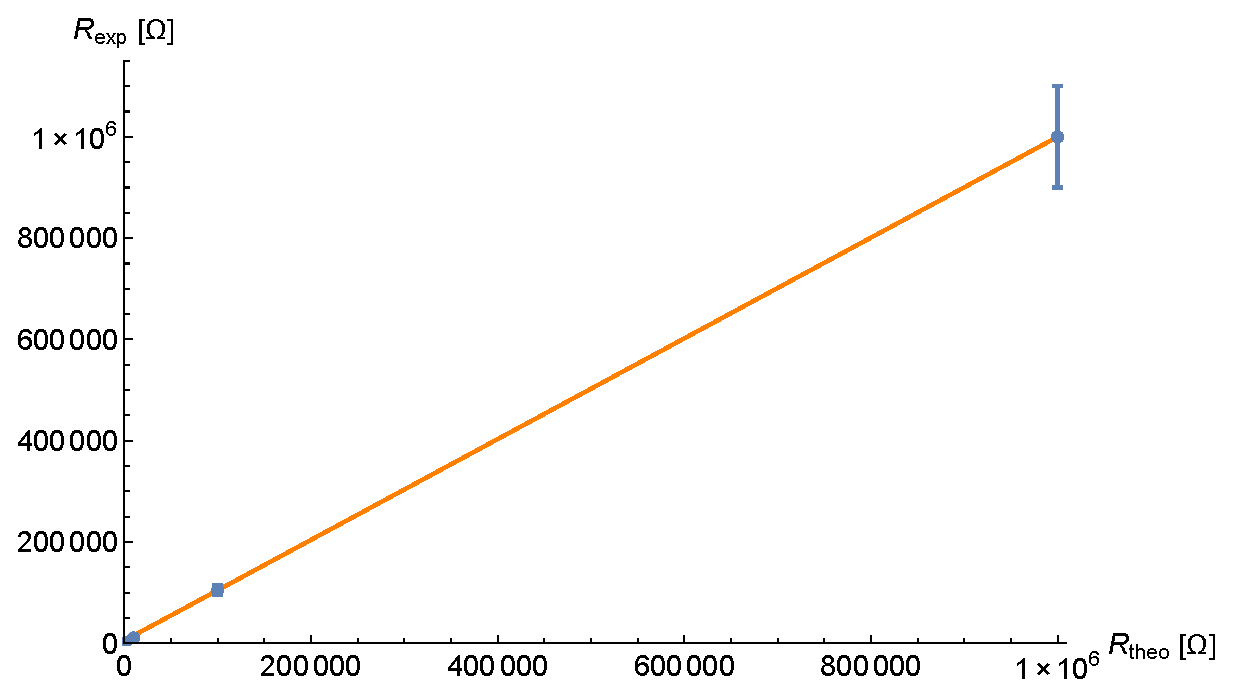
\includegraphics[width=0.5\textwidth]{Berechnung-Bilder/box.eps}
  \caption{
  lineare Regression (Fehlerbalken verzehnfacht). Wir erhalten mit
  Model $R_{exp}=a*R_{theo}+b$:\\
  Steigung:  $a = 0.9944 \pm 3*10^{-4}$\\
  Achsenabschnitt:  $b = (5424 \pm 311) \Omega$
  }
  \label{fig:box}
\end{figure}



%%%%%%%%%%%%%%%%%%%%%%%%%%%%%%%%%%%%%%%%%%%%%%%%%%%%%%%%%%%%%%%%%%%%%%%%%%%%%%%%
\section{Daten und Analyse}
\subsection{Kalibrierung mittels Widerstandsbox}
Die Widerstandsbox mit ihren fest einstellbaren Widerständen bietet uns die
Möglichkeit den Messaufbau zu kalibrieren. Hierzu wurden für die festeingestellten
Widerstände 100 $\Omega$, 1 $k\Omega$, 10 $k\Omega$, 100 $k\Omega$ und 1 $M\Omega$
die Real- und Imaginärteile der Impedanz bei verschiedenen Spannungswerten ermittelt
und durch pythagoräische Addition der Widerstand ermittelt. Als Fehler wurde auf der
Widerstandsbox $0.1\%$ für den Bereich $100\Omega - 10k\Omega$ und $1\%$ für den
Bereich $10k\Omega - 1M\Omega$ gegeben. Aus unseren Messdaten ergibt sich Abb.
\ref{fig:box}. Aus dem Achsenabschnitt können wir den Serienleitwert bestimmen:

  \begin{equation}
    G_S = b^{-1} = (18 \pm 1) mS
  \end{equation}

Die Abweichung der Steigung von 1 werden wir als systematischen Fehler der Messung
interpretieren. Wir müssen also für die folgenden Diagramme den Leitwert wie folgt
korrigieren: $G_{exp} \rightarrow a^{-1} G_{exp}$. Diese Kalibrierung erlaubt es
uns im nächsten Teil die ermittelten Leitwerte korrekt zu ermitteln und ein somit
ein akkurates Ergebnis für die Quantisierung des Leitwertes zu erhalten.


\subsection{Serienleitwert MODFET}
Nun untersuchen wir den MODFET, welchen wir (an einem Messstab befestigt) in
flüssiges Helium getaucht haben. Zusätzlich wird eine Gate-Spannung angelegt,
in deren Abhängigkeit wir der Leitwert bestimmen. Für diesen Teil des Experimentes
verwenden wir zunächst die Struktur G. In Abb. \ref{fig:G} sind 2 der 3 Bereiche
des MODFET gut zu sehen. Im Koordinatenursprung erkennen wir den Sperrbereich des
Transistors in dem kein Drain-Strom fließt, der Transistor sperrt. Im Anschluss
befindet sich der lineare Bereich, in dem sich der Transistor wie ein ohmscher
Widerstand verhält, es gilt: $R = U/I \rightarrow G = I/U$.

\begin{figure}[h]
  \centering
  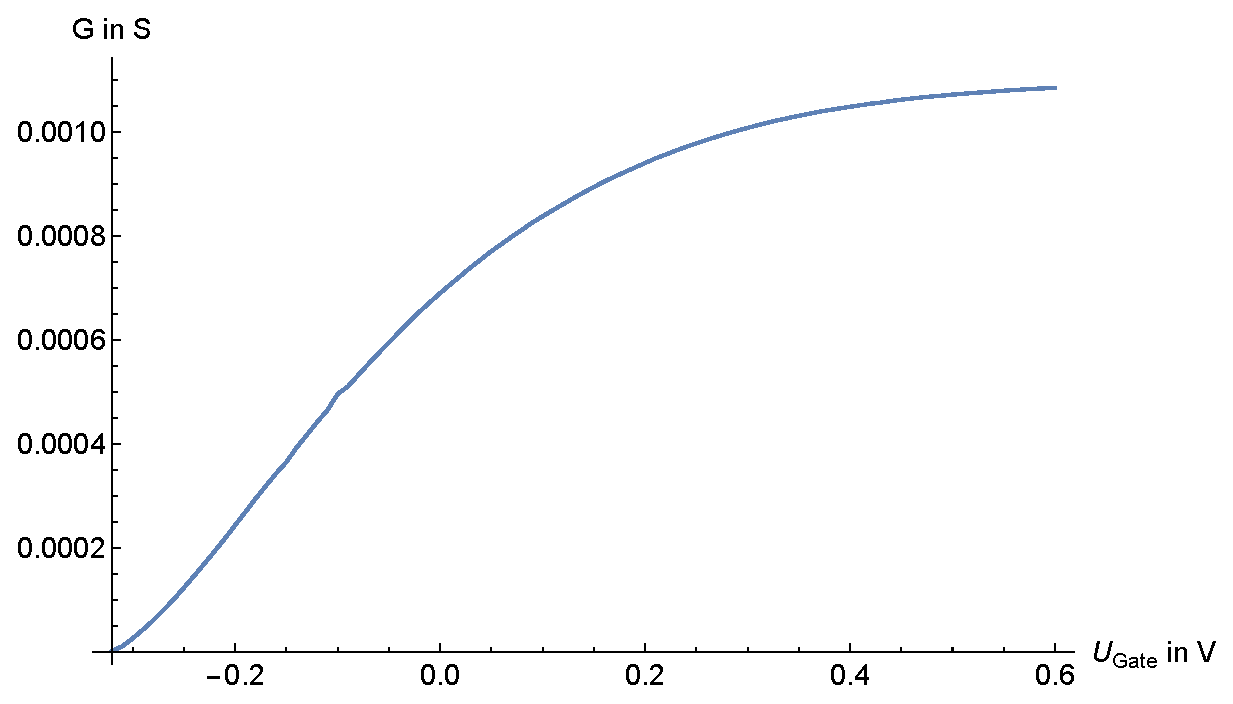
\includegraphics[width=0.5\textwidth]{Berechnung-Bilder/g.eps}
  \caption{Struktur G, Bereiche des Feldeffekttransistors}
  \label{fig:G}
\end{figure}

Der Leitwert nähert sich gegen Ende des linearen
Bereiches einem Maximum an, der dem Serienleitwert entspricht. In diesem sogenannten
Sättigungsbereich verhält sich der Transistor wie eine nur noch durch die Eingangsspannung
gesteuerte Stromquelle, die Gatespannung ändert den Stromfluss nicht mehr. Der
Sättigungsleitwert ist in Abb. \ref{fig:G} als schwarze Linie gekennzeichnet und
wurde mit $G_{sat} \approx 1.2 mS$ abgeschätzt. Dieser entspricht einem Serienwiderstand
von $R_s \approx 833 \Omega$. Wir verwenden den Serienwiderstand im nächsten Abschnitt
um die Quantisierung des Leitwertes zu plotten.


\subsection{Quantisierter Leitwert}
In diesem Versuchsteil werden wir den quantisierten Leitwert in Abhängigkeit von
der Gatespannung beobachten können. Hierfür entnehmen wir aus \cite{skript11}
den folgenden Zusammenhang:

  \begin{equation}
    R = R_s + R_n
  \end{equation}

Hierbei ist $R = G_{exp}^{-1}$ der Gesamtwiderstand der Schaltung ermittelt aus
dem gemessenen Leitwerten, $R_s$ der Serienwiderstand den wir im vorherigen Teil
ermittelt haben und $R_n = 1/G_n$ mit $G_n = n*\frac{2e^2}{h} $ der
(quantisierte) Widerstand der Struktur. Wir verwenden die Struktur I um den
quantisierten Leitwert nachzuweisen. Wir berechnen ihn nach obiger Gleichung mit:

  \begin{equation}
    G_n = \frac{1}{G_{exp}^{-1}-R_s}
  \end{equation}

Nach Messen der Leitwerte $G_{exp}$ und Korrektur mit dem Serienwiderstand $R_s$
ergibt sich Abb. \ref{fig:I}:

\begin{figure}[h]
  \centering
  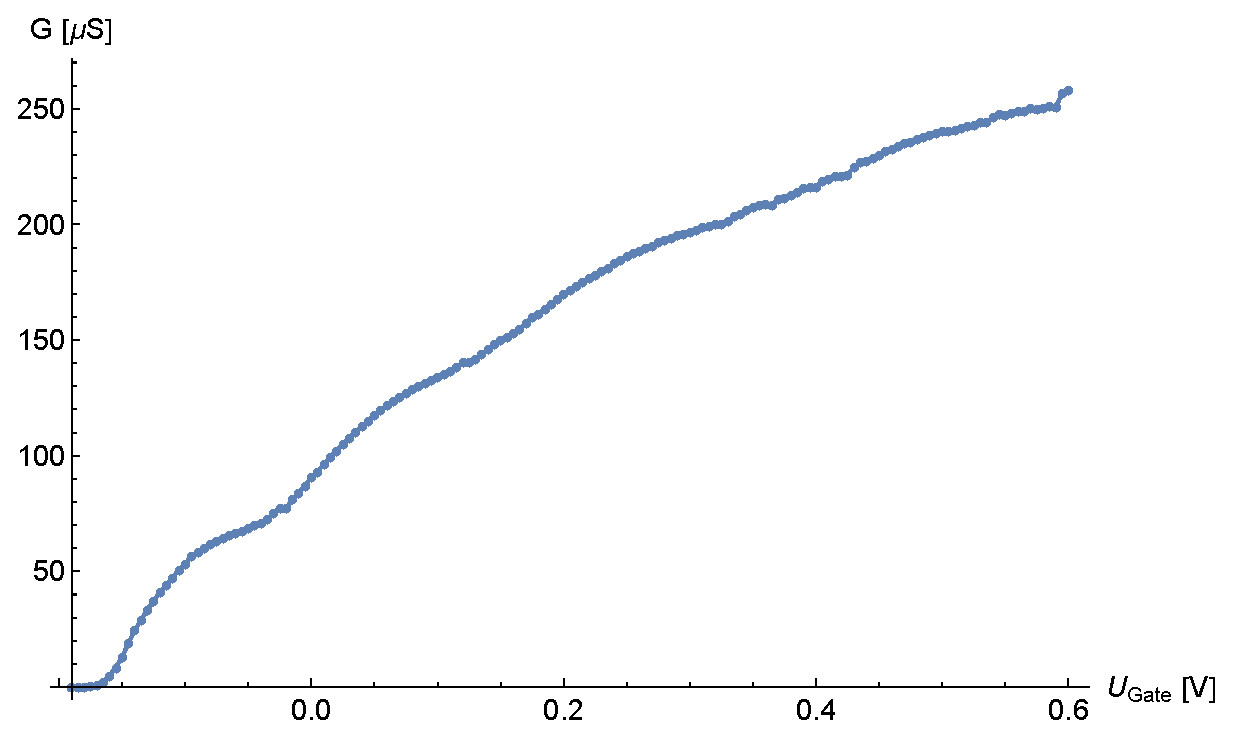
\includegraphics[width=0.5\textwidth]{Berechnung-Bilder/j.eps}
  \caption{Struktur I, quantisierter Leitwert}
  \label{fig:I}
\end{figure}

Als Orientierung sind hier Linien für die Vielfachen von $\frac{2e^2}{h} \approx 77.5 \mu S$
eingezeichnet. Die Ausbildung der Plateaus ist erkennbar, wenn auch nicht stark
ausgeprägt. Als Referenz befinden sich in Anhang A vom Versuchsbetreuer gegebene
Daten einer anderen Struktur, in der die Quantisierung deutlicher erkennbar ist.


\subsection{Fehler und Ergebnisanalyse}
Die schwache Ausprägung der Plateaus kann mehrere Gründe haben. Die wichtigste
Voraussetzung für die Berechnung in Abschnitt I ist die Quantisierung der Elektronen,
d.h. das Ausbilden von Wellen senkrecht zur Bewegungsrichtung. Dies ist nur
gewährleistet, wenn ein ballistischer Transport von Elektronen
stattfindet. Ballistischer Transport heißt, dass die mittlere freie Weglänge der
Elektronen größer ist als die geometrische Ausdehnung der Engstelle. In anderen
Worten: die Streuung der Elektronen muss so gering wie möglich sein! Dies wurde
im Experiment u.A. dadurch gewährleistet, indem die Temperatur auf $T=4K$ abgesenkt
wurde. Allerdings sind weitere Effekte wie die Streuung an Unreinheiten, anderen
Elektronen oder Phononen nicht quantifiziert wurden, womit nicht bestätigt
werden kann, dass die Annahme des ballistischen Transports gerechtfertigt ist.
Diese Überlegungen wollen wir wie folgt illustrieren:
Bei $T=4K$ haben 0.02\% der Elektronen eine Energie, die höher als die
Fermi-Energie ist und verstoßen somit gegen unsere Voraussetzungen. Angesichts der
niedrigen Zahl können wir die Temperatur als Fehler also erst einmal vernachlässigen.
Schwerwiegender ist, dass wir nichts über die Abmessungen des Punktkontakts wissen
und somit nicht rechnerisch nachprüfen können, ob die mittlere freie Weglänge
tatsächlich wesentlich kleiner ist, als die Geometrie des Kontakts.
Neben diesen Unsicherheiten welche aus dem theoretischen Konstrukt entstehen, gibt
es auch experimentelle Unsicherheiten, die nicht berücksichtigt wurden. So wurde
keine Analyse zum Rauschen der Elektronik durchgeführt, welche auf Grund der geringen
Größenordnung der verwandten Spannungen/Ströme einen Einfluss haben könnte.


%%%%%%%%%%%%%%%%%%%%%%%%%%%%%%%%%%%%%%%%%%%%%%%%%%%%%%%%%%%%%%%%%%%%%%%%%%%%%%%%
\section{Schlussfolgerung}

Die Quantisierung des Leitwertes an einem Punktkontakt
konnte in diesem Versuch nachgewiesen werden. Die Ausbildung der Plateaus, welche
uns die Quantisierung anzeigen, sind in Abb. \ref{fig:I} nicht so stark wie gewünscht
bzw. nicht so stark wie in den Referenzdaten in Anhang A (Abb.\ref{fig:l}). Die
möglichen Gründe hierfür, aufgeteilt in theoretisch/konzeptionelle und experimentelle,
wurden bereits in Abschnitt III.4. diskutiert. \\
Zusammenfassend kann man sagen, dass der Versuch ein verhältnismäßig einfach zu
realisierendes und für den Ausführenden interessantes Experiment zeigt, indem man
das quantenmechanische Phänomen der Quantisierung direkt beobachten kann. \\


%%%%%%%%%%%%%%%%%%%%%%%%%%%%%%%%%%%%%%%%%%%%%%%%%%%%%%%%%%%%%%%%%%%%%%%%%%%%%%%%
\bibliography{sample-paper}
\bibliographystyle{prsty}
\begin{thebibliography}{99}
\bibitem{skript11}S. F. Fischer et al. : F-Praktikumsversuch Quantisierter Leitwert von Punktkontakten (Versuchsskript) (2011)
\bibitem{wees88}B. J. van Wees et al. : Quantized Conductance of Point Contacts in a Two-Dimensional Electron Gas, Physical Review Letters Vol. 60 Nr.9 (1988)
\end{thebibliography}


%%%%%%%%%%%%%%%%%%%%%%%%%%%%%%%%%%%%%%%%%%%%%%%%%%%%%%%%%%%%%%%%%%%%%%%%%%%%%%%%
\appendix

\section{Referenzdaten und Grafiken}
Vom Versuchsbetreuer wurden uns noch die Daten der folgenden Grafiken gegeben.

\begin{figure}[h]
  \centering
  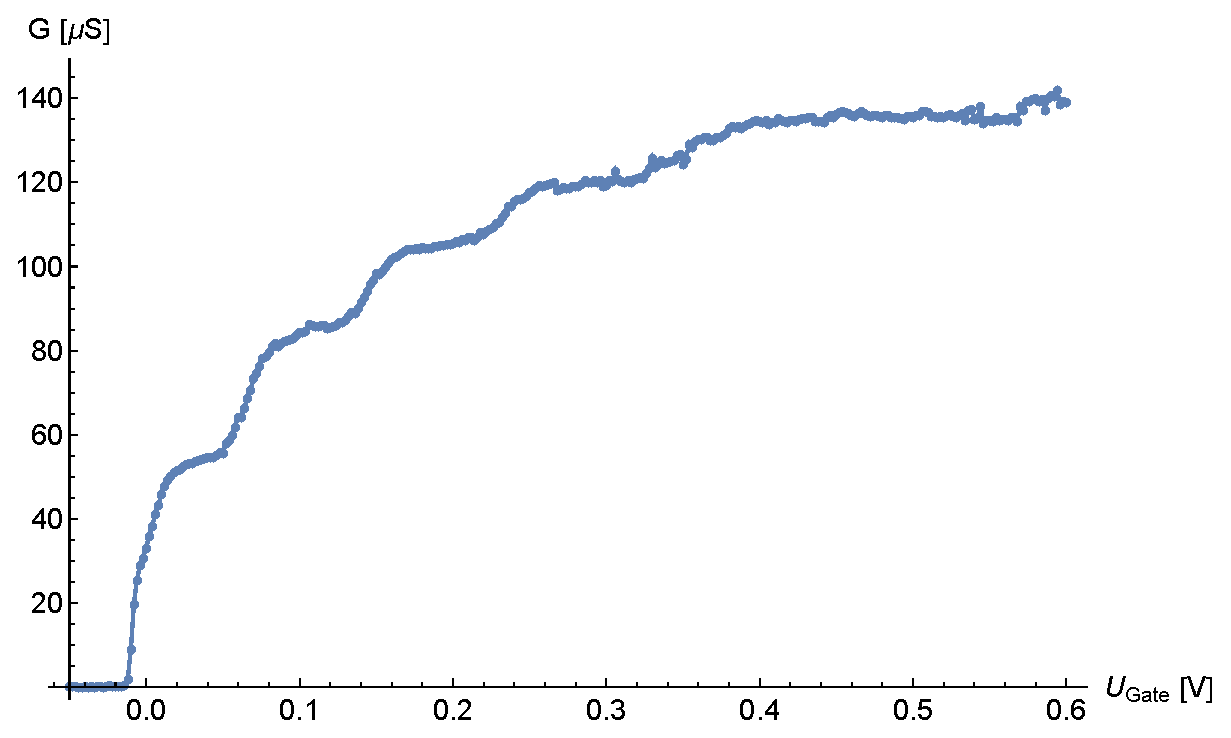
\includegraphics[width=0.5\textwidth]{Berechnung-Bilder/l.eps}
  \caption{Struktur L, quantisierter Leitwert}
  \label{fig:l}
\end{figure}

\newpage
Es sind nur die experimentell ermittelten Leitwerte $G_{exp}$ dargestellt, da uns
keine weiteren Informationen (insbesondere die Kalibrierung mit Widerstandsbox)
vorliegen. Nichtsdestotrotz ist die Quantisierung des Leitwerts in Abb. \ref{fig:l}
und Abb. \ref{fig:lfein} deutlicher erkennbar, als dies bei unseren Daten der Fall ist.

\begin{figure}[h]
  \centering
  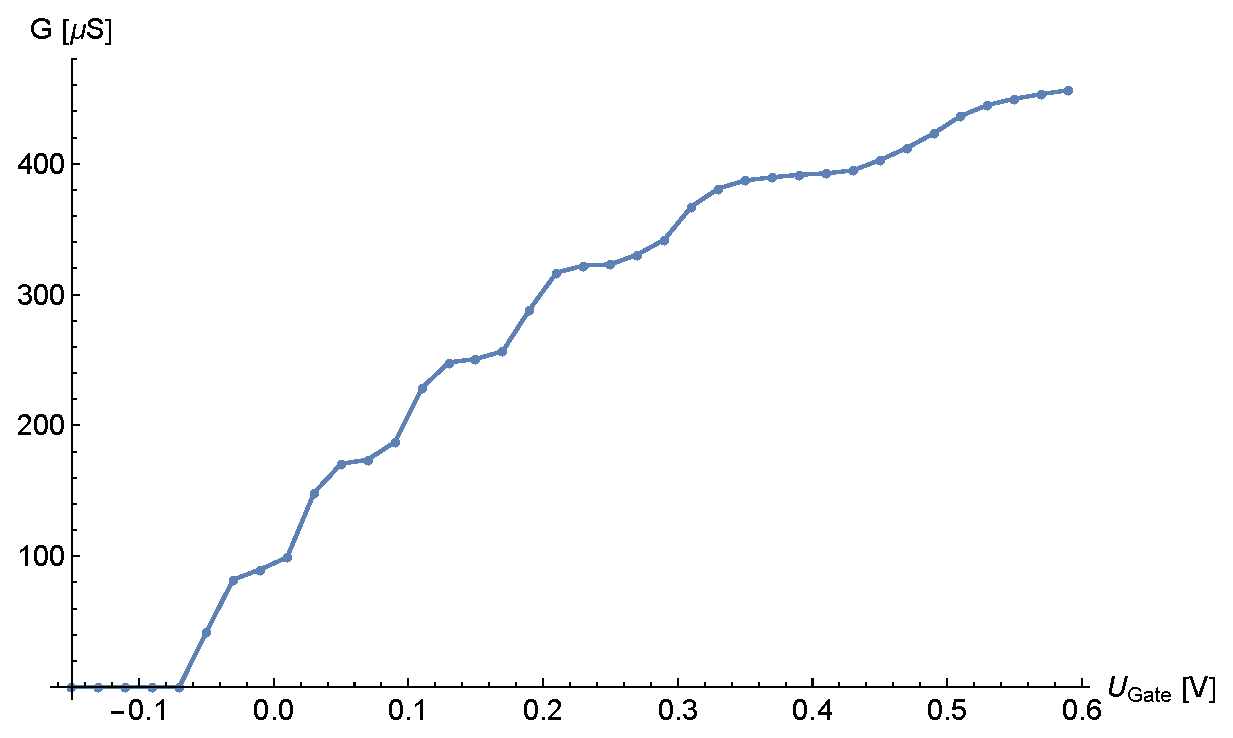
\includegraphics[width=0.5\textwidth]{Berechnung-Bilder/lfein.eps}
  \caption{Struktur Lfein, quantisierter Leitwert}
  \label{fig:lfein}
\end{figure}


%%%%%%%%%%%%%%%%%%%%%%%%%%%%%%%%%%%%%%%%%%%%%%%%%%%%%%%%%%%%%%%%%%%%%%%%%%%%%%%%


\end{document}
